% ==============================================================================
% VLIZ Scientific Research Poster - Marine Term Translations (MTT)
% ==============================================================================
% Prepared for Scientific Audience: Term Translators & Ontology Stewards
% Template: VLIZ Institutional tikzposter (Sea-Teal Banner #91C8CD, Wave Logo)
% Layout Paradigm: Top Hero Architecture & 3-Column Dual-Persona Evidence
% Empirical Design: Khadka & Peeters (2024) MAR Exemplary Tier (250-400 words)
% Visual Enhancements: Aligned Bottom Baselines & Tight Infographic Framing
% ==============================================================================

\documentclass[
  25pt,
  a0paper,
  portrait,
  margin=0mm,
  innermargin=15mm,
  blockverticalspace=8mm,
  colspace=10mm,
  subcolspace=8mm
]{tikzposter}

\usepackage{graphicx}
\graphicspath{{assets/}{posters/marine-term-translations/assets/}{posters/vliz-poster/assets/}{templates/posters/assets/}}
\usepackage{amsmath,amssymb}
\usepackage{qrcode}
\usepackage{hyperref}
\usepackage{tikz}
\usetikzlibrary{positioning,calc,arrows.meta}
\usepackage{tcolorbox}

% ------------------------------------------------------------------------------
% VLIZ Institutional Color Palette
% ------------------------------------------------------------------------------
\definecolor{vlizBanner}{HTML}{91C8CD}       % Exact Sea-teal from template
\definecolor{vlizTeal}{HTML}{31B7BC}         % Vibrant teal subtitle
\definecolor{vlizNavy}{HTML}{3057A5}         % Corporate Navy
\definecolor{vlizCharcoal}{HTML}{231F20}     % Dark Charcoal author font
\definecolor{vlizSlateText}{HTML}{1E293B}    % Main body text
\definecolor{vlizSlateMuted}{HTML}{64748B}   % Muted text
\definecolor{vlizCardBg}{HTML}{FFFFFF}       % White card background
\definecolor{vlizHeroBg}{HTML}{F8FAFC}       % Soft slate hero card background
\definecolor{vlizBorder}{HTML}{CBD5E1}       % Card border
\definecolor{vlizLightTeal}{HTML}{E6F7F8}   % Light teal accent for pipeline

% Set custom tikzposter style
\definecolorstyle{VLIZStyle}{
  \definecolor{colorOne}{HTML}{3057A5}
  \definecolor{colorTwo}{HTML}{31B7BC}
  \definecolor{colorThree}{HTML}{91C8CD}
}{
  \colorlet{backgroundcolor}{white}
  \colorlet{framecolor}{white}
  \colorlet{titlefgcolor}{vlizNavy}
  \colorlet{titlebgcolor}{white}
  \colorlet{blocktitlebgcolor}{white}
  \colorlet{blocktitlefgcolor}{vlizNavy}
  \colorlet{blockbodybgcolor}{vlizCardBg}
  \colorlet{blockbodyfgcolor}{vlizSlateText}
}

\usetheme{Default}
\usecolorstyle{VLIZStyle}
\tikzposterlatexaffectionproofoff

% Custom block style: Clean card with subtle border and crisp typography
\defineblockstyle{VLIZBlock}{
  titlewidthscale=1.0, bodywidthscale=1.0,
  titleoffsetx=0pt, titleoffsety=0pt, bodyoffsetx=0pt, bodyoffsety=0pt,
  bodyverticalshift=0pt, roundedcorners=14, linewidth=2pt,
  titleinnersep=4mm, bodyinnersep=6mm
}{
  \draw[color=vlizBorder, fill=blockbodybgcolor, rounded corners=14, line width=2pt]
    (blockbody.south west) rectangle (blocktitle.north east);
}
\useblockstyle{VLIZBlock}

% Suppress default centered title
\title{}
\author{}
\institute{}

\begin{document}

% ==============================================================================
% 1. TOP BANNER (Official VLIZ Vector Header)
% ==============================================================================
\fill[vlizBanner] (-0.5\paperwidth, 0.5\paperheight)
  rectangle (0.5\paperwidth, {0.5\paperheight - 0.115\paperheight});

% Vector VLIZ Logo
\node[anchor=west, inner sep=0pt] at ({-0.5\paperwidth + 0.088\paperwidth}, {0.5\paperheight - 0.0575\paperheight}) {
  
\includegraphics[height=0.065\paperheight]{vliz_logo.png}
};

% Sharp Native Vector Typography for URL
\node[anchor=east, inner sep=0pt] at ({0.5\paperwidth - 0.088\paperwidth}, {0.5\paperheight - 0.0575\paperheight}) {
  {\color{vlizNavy}\sffamily\bfseries\fontsize{34pt}{40pt}\selectfont vliz.be}
};

% ==============================================================================
% 2. TITLE & AUTHORS SECTION (Left-Aligned Institutional Branding)
% ==============================================================================
\node[anchor=north west, text width=0.84\paperwidth, align=flush left, inner sep=0pt]
  at ({-0.5\paperwidth + 0.088\paperwidth}, {0.5\paperheight - 0.128\paperheight}) {
  % Subtitle / Venue & Audience Callout
  {\color{vlizTeal}\bfseries\LARGE MULTILINGUAL MARINE VOCABULARIES \quad $\vert$ \quad mtt.vliz.be \quad $\vert$ \quad FOR TRANSLATORS \& ONTOLOGY STEWARDS \par}
  \vspace{0.3cm}
  % Main Title
  {\color{vlizNavy}\bfseries\fontsize{44pt}{52pt}\selectfont Marine Term Translations (MTT): Continuous LDES Ingestion, Collaborative Multilingual Curation, and Downstream Vocabulary Widgets \par}
  \vspace{0.35cm}
  % Author
  {\color{vlizCharcoal}\bfseries\LARGE Cedric Decruw \par}
  \vspace{0.2cm}
  % Affiliations & Contact
  {\color{vlizSlateMuted}\large Flanders Marine Institute (VLIZ), InnovOcean Campus, 8400 Oostende, Belgium \quad $\vert$ \quad cedric.decruw@vliz.be \quad $\vert$ \quad ORCID: 0000-0001-6387-5988 \par}
};

% ==============================================================================
% Set starting vertical position for tikzposter blocks
% ==============================================================================
\makeatletter
\setlength{\TP@blocktop}{0.5\textheight - 275mm}
\makeatother

% ==============================================================================
% 3. HERO INFOGRAPHIC BANNER: TIGHT CONTINUOUS LDES LIFECYCLE
% ==============================================================================
\block{}{
  \centering
  \vspace{-0.2cm}
  {\color{vlizNavy}\bfseries\huge Central Architecture: Continuous LDES Ingestion, MTT Curation \& vocab.vliz.be Widgets \par}
  \vspace{0.1cm}
  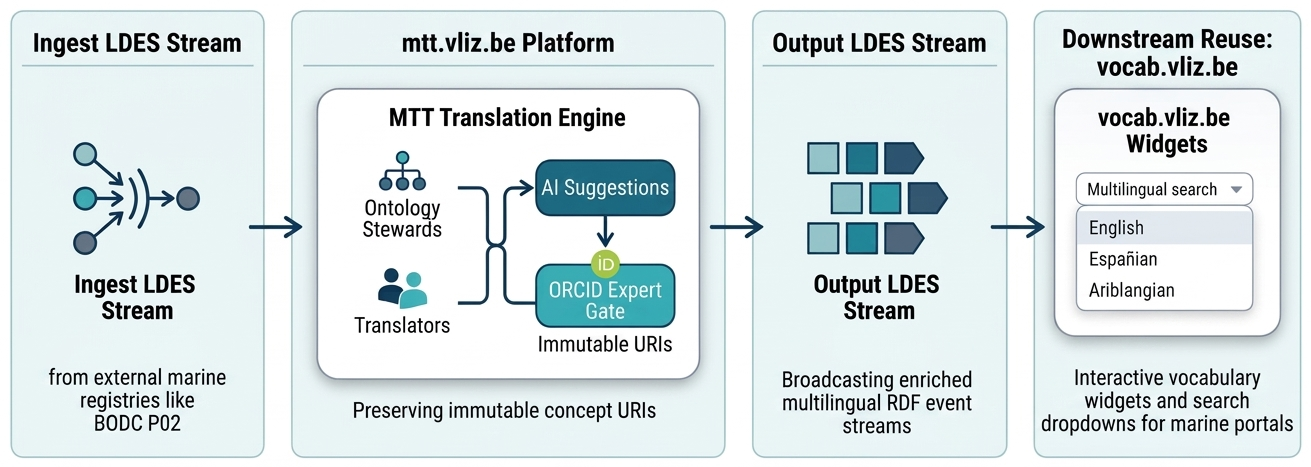
\includegraphics[width=0.99\linewidth]{mtt-ldes-continuous-pipeline.png}\\[-0.05cm]
  {\color{vlizSlateMuted}\large \textbf{Figure 1:} Continuous semantic pipeline: Upstream LDES ingestion $\rightarrow$ \texttt{mtt.vliz.be} translation workbench (AI suggestions + ORCID peer gate) $\rightarrow$ Outgoing LDES publication $\rightarrow$ Live reuse in \texttt{vocab.vliz.be} widgets.}
  \vspace{-0.1cm}
}

% ==============================================================================
% 4. SUPPORTING 3-COLUMN EVIDENCE GRID (Audience-Targeted Pillars)
% ==============================================================================
\begin{columns}
  % ---- Column 1: For Ontology Stewards & Ingestion ----
  \column{0.333}
  
  \block{1. For Ontology Stewards: Ingestion \& Sync}{
    \textbf{Operational Context:}
    \begin{itemize}\setlength{\itemsep}{2pt}
      \item Marine registries (e.g. BODC P02, SeaDataNet) publish authoritative terms in English.
      \item Static snapshot downloads cause sync latency, manual drift, and URI churn.
    \end{itemize}
    
    \vspace{0.15cm}
    \textbf{Research Question (RQ):}
    \begin{itemize}\setlength{\itemsep}{2pt}
      \item \textit{How to ingest ontologies and enrich them multilingually while preserving concept identities?}
    \end{itemize}
    
    \vspace{0.15cm}
    \textbf{Hypothesis \& Prediction:}
    \begin{itemize}\setlength{\itemsep}{2pt}
      \item \textit{Streaming LDES ingestion with decoupled concept modeling eliminates sync lag without URI churn.}
    \end{itemize}
    
    \vspace{0.2cm}
    \textbf{Platform Value for Stewards:}
    \vspace{0.12cm}

    \begin{tcolorbox}[colback=vlizLightTeal,colframe=vlizBanner,arc=4mm,boxrule=1.5pt,left=5mm,right=5mm,top=3mm,bottom=3mm]
      {\color{vlizNavy}\bfseries Continuous LDES Ingestion}\\[2pt]
      {\small Ingests upstream LDES event feeds, tracking term updates incrementally without bulk downloads.}
    \end{tcolorbox}
    \vspace{0.12cm}
    \begin{tcolorbox}[colback=vlizLightTeal,colframe=vlizBanner,arc=4mm,boxrule=1.5pt,left=5mm,right=5mm,top=3mm,bottom=3mm]
      {\color{vlizNavy}\bfseries Zero Concept URI Churn}\\[2pt]
      {\small Persistent concept URIs remain immutable as multilingual labels evolve, ensuring stable references.}
    \end{tcolorbox}
    \vspace{0.12cm}
    \begin{tcolorbox}[colback=vlizLightTeal,colframe=vlizBanner,arc=4mm,boxrule=1.5pt,left=5mm,right=5mm,top=3mm,bottom=3mm]
      {\color{vlizNavy}\bfseries Institutional Data Sovereignty}\\[2pt]
      {\small 100\% self-hostable open stack (React, Node.js, PostgreSQL) deployable on local infrastructure.}
    \end{tcolorbox}
    \vspace{0.12cm}
    \begin{tcolorbox}[colback=vlizHeroBg,colframe=vlizBorder,arc=4mm,boxrule=1.5pt,left=5mm,right=5mm,top=3mm,bottom=3mm]
      {\color{vlizNavy}\bfseries Standards-Based Interoperability}\\[2pt]
      {\small Dual export pathways: CSV, SKOS, JSON-LD, and continuous Linked Data Event Streams.}
    \end{tcolorbox}
  }

  % ---- Column 2: For Term Translators & Curation ----
  \column{0.334}
  
  \block{2. For Translators: Curation \& Credit}{
    \textbf{The Translation Bottleneck:}
    \begin{itemize}\setlength{\itemsep}{2pt}
      \item Domain experts are deterred by complex semantic tools (Prot\'eg\'e, raw RDF) and unstructured spreadsheets.
      \item Linguistic translations often go uncredited in academic pipelines.
    \end{itemize}
    
    \vspace{0.18cm}
    \textbf{The mtt.vliz.be Workbench:}
    \vspace{0.12cm}

    \begin{tcolorbox}[colback=vlizHeroBg,colframe=vlizBorder,arc=4mm,boxrule=1.5pt,left=5mm,right=5mm,top=3.0mm,bottom=3.0mm]
      {\color{vlizNavy}\bfseries 1. Side-by-Side Comparison UI}\\[2pt]
      {\small Distraction-free browser interface comparing source terms directly with translations.}
    \end{tcolorbox}
    \vspace{0.12cm}
    \begin{tcolorbox}[colback=vlizHeroBg,colframe=vlizBorder,arc=4mm,boxrule=1.5pt,left=5mm,right=5mm,top=3.0mm,bottom=3.0mm]
      {\color{vlizNavy}\bfseries 2. AI-Assisted Candidate Drafting}\\[2pt]
      {\small Contextual suggestions accelerate initial drafting velocity by $2\times$ across batches.}
    \end{tcolorbox}
    \vspace{0.12cm}
    \begin{tcolorbox}[colback=vlizHeroBg,colframe=vlizBorder,arc=4mm,boxrule=1.5pt,left=5mm,right=5mm,top=3.0mm,bottom=3.0mm]
      {\color{vlizNavy}\bfseries 3. Human-in-the-Loop Review Gate}\\[2pt]
      {\small Machine suggestions remain provisional until validated by domain specialists.}
    \end{tcolorbox}
    \vspace{0.12cm}
    \begin{tcolorbox}[colback=vlizHeroBg,colframe=vlizBorder,arc=4mm,boxrule=1.5pt,left=5mm,right=5mm,top=3.0mm,bottom=3.0mm]
      {\color{vlizNavy}\bfseries 4. Citable ORCID Attribution}\\[2pt]
      {\small Every approved label is bound to ORCID, guaranteeing citable academic credit.}
    \end{tcolorbox}

    \vspace{0.18cm}
    \textbf{Governance:} Role-aware permissions and complete version audit logs.

    \vspace{0.12cm}
    \begin{tcolorbox}[colback=vlizLightTeal,colframe=vlizTeal,arc=4mm,boxrule=1.5pt,left=5mm,right=5mm,top=3.0mm,bottom=3.0mm]
      {\color{vlizNavy}\bfseries Community Participation \& Impact}\\[2pt]
      {\small \textbf{Translators}: Review and curate terminology in your native language.\\
      \textbf{Stewards}: Register ontologies for automated continuous ingestion.}
    \end{tcolorbox}
    \vspace*{1.8mm}
  }

  % ---- Column 3: Downstream Impact & vocab.vliz.be Widgets ----
  \column{0.333}
  
  \block{3. Outgoing LDES \& vocab.vliz.be Widgets}{
    \textbf{Downstream Delivery Pipeline:}
    \vspace{0.12cm}

    \begin{tcolorbox}[colback=vlizLightTeal,colframe=vlizBanner,arc=4mm,boxrule=1.5pt,left=5mm,right=5mm,top=2.8mm,bottom=2.8mm]
      {\color{vlizNavy}\bfseries Outgoing LDES Stream Broadcast}\\[2pt]
      {\small Approved translations emitted as immutable RDF event feeds, eliminating bulk snapshot downloads.}
    \end{tcolorbox}
    \vspace{0.12cm}
    \begin{tcolorbox}[colback=vlizLightTeal,colframe=vlizBanner,arc=4mm,boxrule=1.5pt,left=5mm,right=5mm,top=2.8mm,bottom=2.8mm]
      {\color{vlizNavy}\bfseries vocab.vliz.be Widgets Endgoal}\\[2pt]
      {\small Curated terms power drop-in autocomplete and search widgets across marine portals.}
    \end{tcolorbox}

    \vspace{0.15cm}
    \textbf{Empirical Results (BODC P02 Beta):}
    \vspace{0.12cm}

    % Stat Metric Callout Badges
    \noindent
    \begin{minipage}{0.48\linewidth}
      \begin{tcolorbox}[colback=vlizLightTeal,colframe=vlizNavy,arc=4mm,boxrule=2pt,halign=center,top=3mm,bottom=3mm]
        {\color{vlizNavy}\bfseries\fontsize{32pt}{36pt}\selectfont 25\%}\\[2pt]
        {\small P02 Translated}
      \end{tcolorbox}
    \end{minipage}\hfill
    \begin{minipage}{0.48\linewidth}
      \begin{tcolorbox}[colback=vlizHeroBg,colframe=vlizTeal,arc=4mm,boxrule=2pt,halign=center,top=3mm,bottom=3mm]
        {\color{vlizTeal}\bfseries\fontsize{32pt}{36pt}\selectfont 2$\times$}\\[2pt]
        {\small Drafting Speed}
      \end{tcolorbox}
    \end{minipage}

    \vspace{0.15cm}
    \begin{itemize}\setlength{\itemsep}{2pt}
      \item \textbf{Supported Hypothesis:} Zero URI churn; continuous sync proven.
      \item \textbf{1 Study Limitation:} Throughput bounded by reviewer bandwidth.
      \item \textbf{Actionable Future Direction:} Deploy automated confidence triage.
    \end{itemize}

    \vspace{0.12cm}
    \begin{tcolorbox}[colback=vlizLightTeal,colframe=vlizNavy,arc=4mm,boxrule=1.5pt,halign=center,top=2.5mm,bottom=2.5mm]
      {\color{vlizNavy}\bfseries Test the Live Platform \& Widgets}\\[3pt]
      \qrcode[height=4.3cm]{https://mtt.vliz.be/}\\[3pt]
      {\small \textbf{mtt.vliz.be}}
    \end{tcolorbox}
    \vspace*{0.18cm}
  }
\end{columns}

% ==============================================================================
% 5. FOOTER (Institutional Acknowledgments & AI Disclosure)
% ==============================================================================
\block{}{
  \footnotesize
  \begin{minipage}{0.74\linewidth}
    \textbf{References:} [1] Wilkinson et al. (2016). Sci. Data. \quad [2] BODC (2024). NERC P02. \quad [3] Van de Vyvere et al. (2022). LDES.\\
    \textbf{AI Disclosure:} Assisted with language polish and schematic layout; system design and evaluation by the author.
  \end{minipage}%
  \hfill
  \begin{minipage}{0.24\linewidth}
    \raggedleft
    \textbf{Flanders Marine Institute (VLIZ)}\\
    \texttt{mtt.vliz.be} \quad $\vert$ \quad \texttt{vocab.vliz.be}
  \end{minipage}
}

\end{document}
